\section{Results and Specific Discussion}

\subsection{Improvements to the Slimplectic Integrator and their Physical Applications}
\label{sec:results-si}

\begin{figure}[t]
  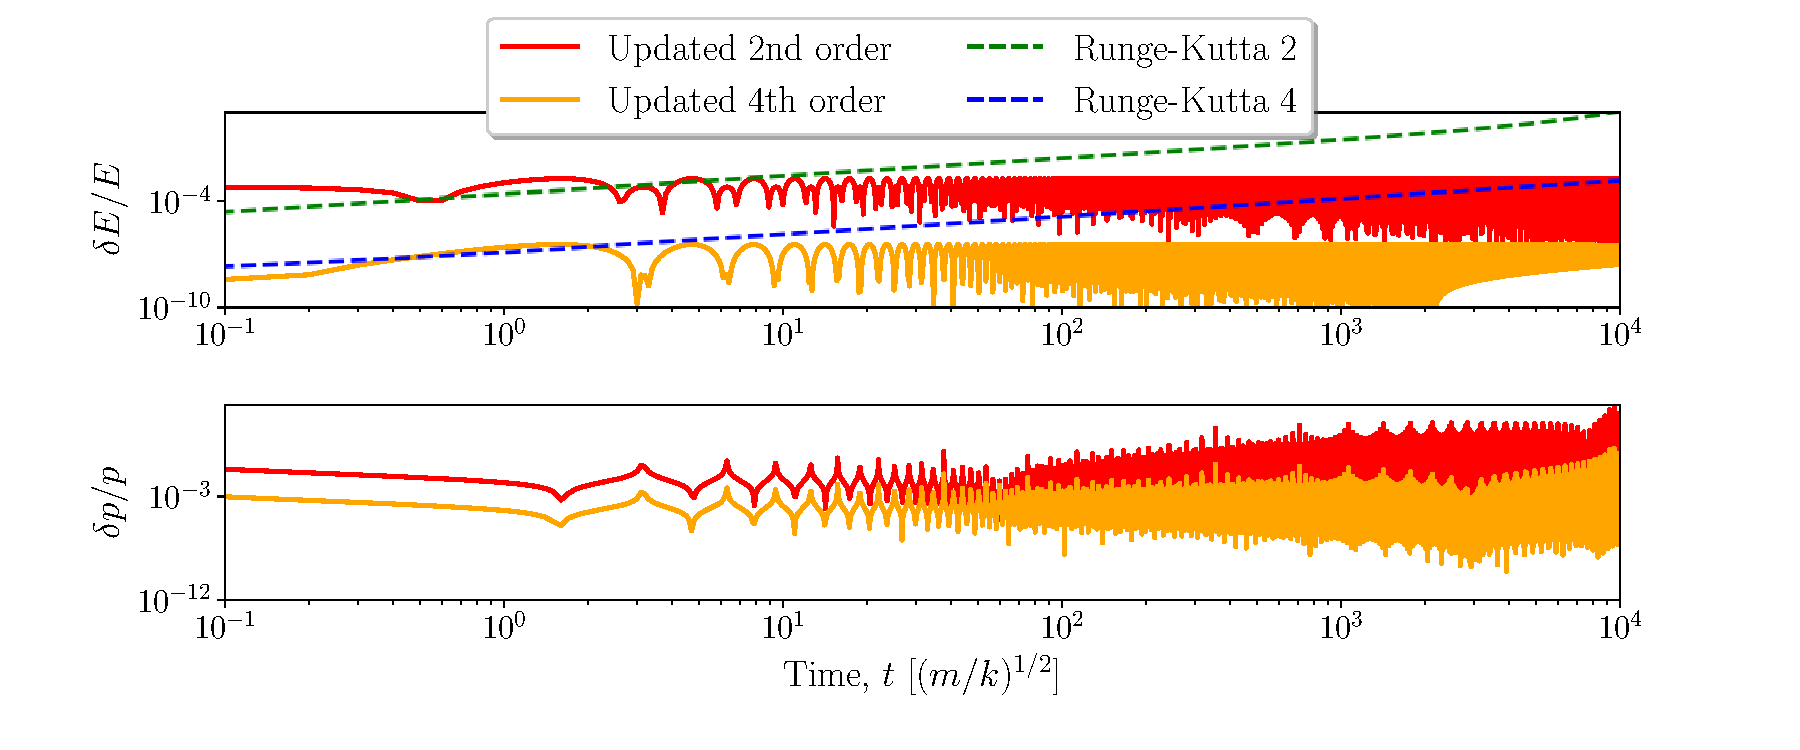
\includegraphics[width=\columnwidth]{figures/dho_energy_momenta_fractional_err.pdf}
  \caption{A comparison of the error in the energy, top, and momenta, bottom, as a fraction of the known analytic solution of the system, of the \updimpl{} simulating a damped harmonic oscillator. One can clearly observe that the fractional energy error is bounded and displays the oscillating behaviour that we expect from previous work, whereas the momenta error does not display such behaviour. This plot is based off its equivalent in the original paper \cite[Figure 2, bottom]{tsangSLIMPLECTICINTEGRATORSVARIATIONAL2015}.}
\label{fig:dho_energy_bounds}
\end{figure}

As discussed we first verify that the \updimpl{} retains required fractional error bounds of the formal method. This can be seen in \fref{fig:dho_energy_bounds} where the fractional error of the \updimpl{} with respect to that of the true analytic solution is compared directly against that of Runge-Kutta order 2 and 4. We clearly observe that the fractional energy error remains bounded across the timeframe of iteration.
This successfully replicated the behaviour of the original implementation to an absolute root mean squared residual over the simulation duration of $\Delta = 1.42 \times 10^{-13}$ and $\Delta = 4.50 \times 10^{-12}$ for $r = 2$ and $r = 4$ respectively.
This is not the case for the fractional momenta error however as fixed-time-step variational methods such as those implemented cannot be both slimplectic-momentum and momentum-energy preserving \cite{zhongLiePoissonHamiltonJacobiTheory1988}.

\begin{figure}[t]
  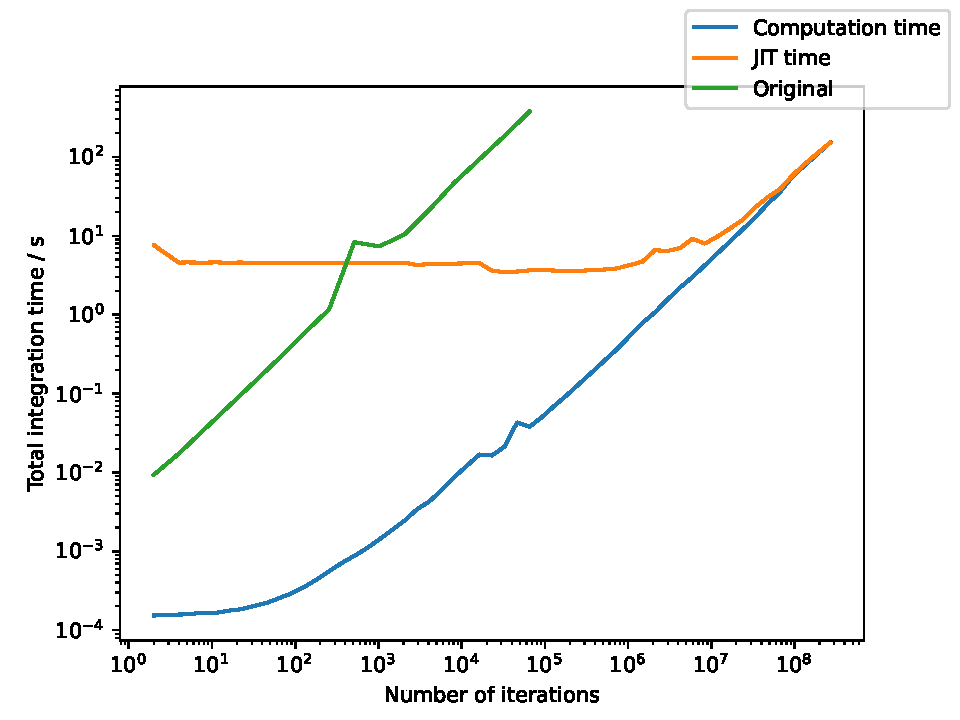
\includegraphics[width=\columnwidth]{figures/dho_n_runtime.pdf}
  \caption{A comparison of running a damped harmonic oscillator system for various numbers of iterations, with $r = 2, \Delta t = 0.1$. The \updimpl{} runtime is split into two components where \ensquote{JIT time} represents the one time fixed cost of compiling the function (see \sref{sec:intro-autodiff}) and \enquote{Computation time} represents the actual time spent on computation.
  Each value is the mean of 4 runs, with the \orgimpl{} being cut off early due after $> 20$ minutes runtime for the next sample.}
  \label{fig:dho-n-runtime}
\end{figure}

\begin{figure}[t]
  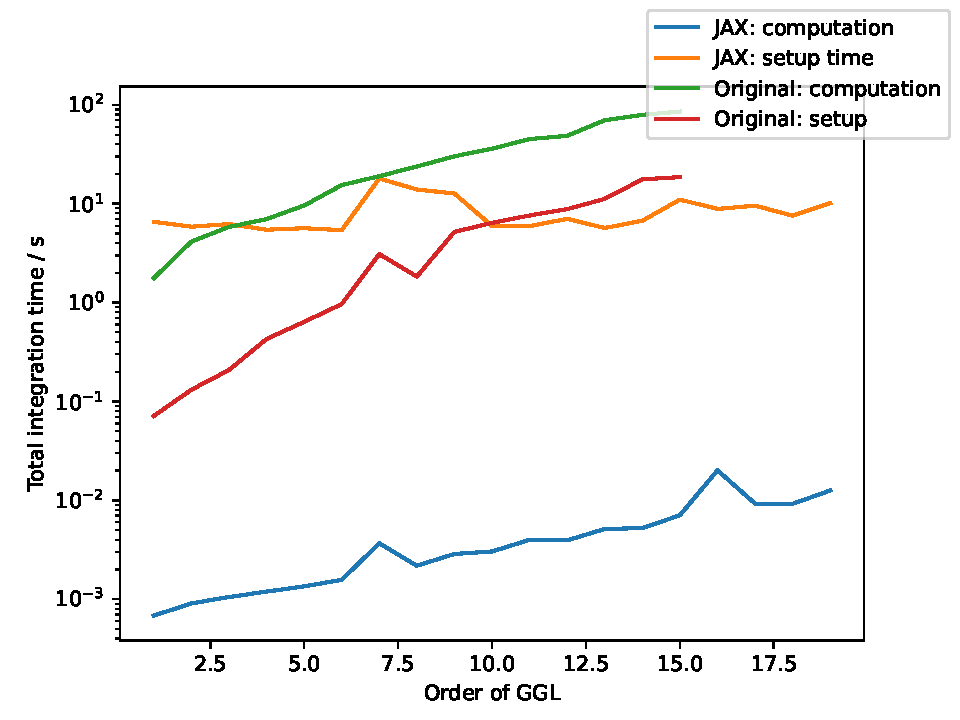
\includegraphics[width=\columnwidth]{figures/dho_r_runtime.pdf}
  \caption{A comparison of running a damped harmonic oscillator system for various values of $r$, the order of the GGL quadrature, with $\Niter = 500, \Delta t = 0.1$. Each result being the mean of 4 independent runs.
	For both implementations we split the overall time into setup and computation as changing the method order requires re-discretising the Lagrangian and thus non-trivial work under both implementations.}
  \label{fig:dho-r-runtime}
\end{figure}

Next we explored the time complexity of the system in terms of the iteration count, $N_{\text{iter}}$, and GGL quadrature order, $r$. These are important to physical applications as they determine the limits of iteration accuracy when iterating over large timescales -- with error scaling as $(\Delta t)^{2r + 2}$ and total timeframe being $N_{\text{iter}} \Delta t$.

Focusing first on the time complexity in $N_{\text{iter}}$ as shown in \fref{fig:dho-n-runtime}, we note that that the computation time of the \updimpl{} is much lower than that of the \orgimpl{}, with the \updimpl{} growing as $\Or((\Niter)^a)$ where $a = 1.0140 \pm 0.0042$. 
In addition we note that the fixed cost JIT compilation remains roughly constant until $10^7$ iterations after which it begins to grow linearly.

This pattern is seen also in \fref{fig:dho-r-runtime} when investigating the time-complexity in the order of the method. Again the JIT time remains roughly constant across the domain tested, and though it starts out initially higher than than the \orgimpl{}'s setup costs, the \orgimpl{}'s computation time quickly swamps this fixed cost.
Similar to the behaviour in $\Niter$, the computation time for the \updimpl{} is also linear $r$ , remaining insignificant in the overall runtime. This is in comparison with the \orgimpl{} where the setup time grows as $\Or(r^n)$ with $n = {2.31 \pm 0.15}$ and the computation time as $\Or(r^m)$ with $m={1.490 \pm 0.070}$.

It should be noted that while increasing the order of the method will increase the precision, at higher orders we start encountering limitations with the fixed precision \texttt{float64} type used for calculation in the \updimpl{} compared the the arbitrary precision numerics employed in the \orgimpl{}.
Still however this represents an overall improvement in accuracy in physically meaningful simulations as the required precision could be more readily attained by decreasing $\Delta t$ rather than increasing $r$, avoiding the blowup of runtime observed in the \orgimpl{}, or the degradation of precision at high $r$ in the \updimpl{}. This is discussed further in \sref{sec:results-si}


\subsection{Loss Functions and Optimisation}
\label{sec:res-lf}

\todo{this first sentence needs re-wording}
Moving now onto the loss function and choice of Lagrangian embedding function. We explored a number of loss functions through a combination of gradient-descent and visual inspection.

A wide number of loss functions were tested, however focusing on those surrounding systems of harmonic oscillators, we settled on DHO system specific embedding shown in equation \eqref{eq:dho-sys-embedding}, labelled DHO 3.
As well an adaption where an additional embedding parameter $\alpha$ was introduced as pre-factor on the entire non-conservative Lagrangian $\Lambda$, labelled DHO 4. 
These were paired with a number of simple loss functions, \tref{table:loss-fns}, drawing from physical knowledge and existing convention for neural network loss functions.

First we perform a visual inspection of the \enquote{Simple RMS} loss function at various scales with both embedding functions, as seen in \fref{fig:loss-function-behaviour}. Here we observe mild non-convexity around the minima, as impulse like behaviour around the highly non-physical $m = 0$ point.

To test how this mild non-convexity translates into optimisation performance we subject a number of combinations to empirical optimisation tests where we attempt to attain a known true embedding from a number of random initial embedding values. \Tref{table:optimisation-results} (see caption for details) shows that that the addition of the global pre-factor $\alpha$ substantially increases the probability of successful convergence.  In addition we see that both the $\vbq$ and $\pi$ values are important in the fitting process from the complete lack of convergence when only $\pi$ is included, and that their relative weight seems to be of little importance at this stage.

This is promising as, while optimisation directly in the embedding space is a strictly simpler problem than with respect to the parameters of an associated neural network, it suggests that this mild non-convexity observed during visual inspect is an obstacle we can overcome.

\begin{figure*}[t]
  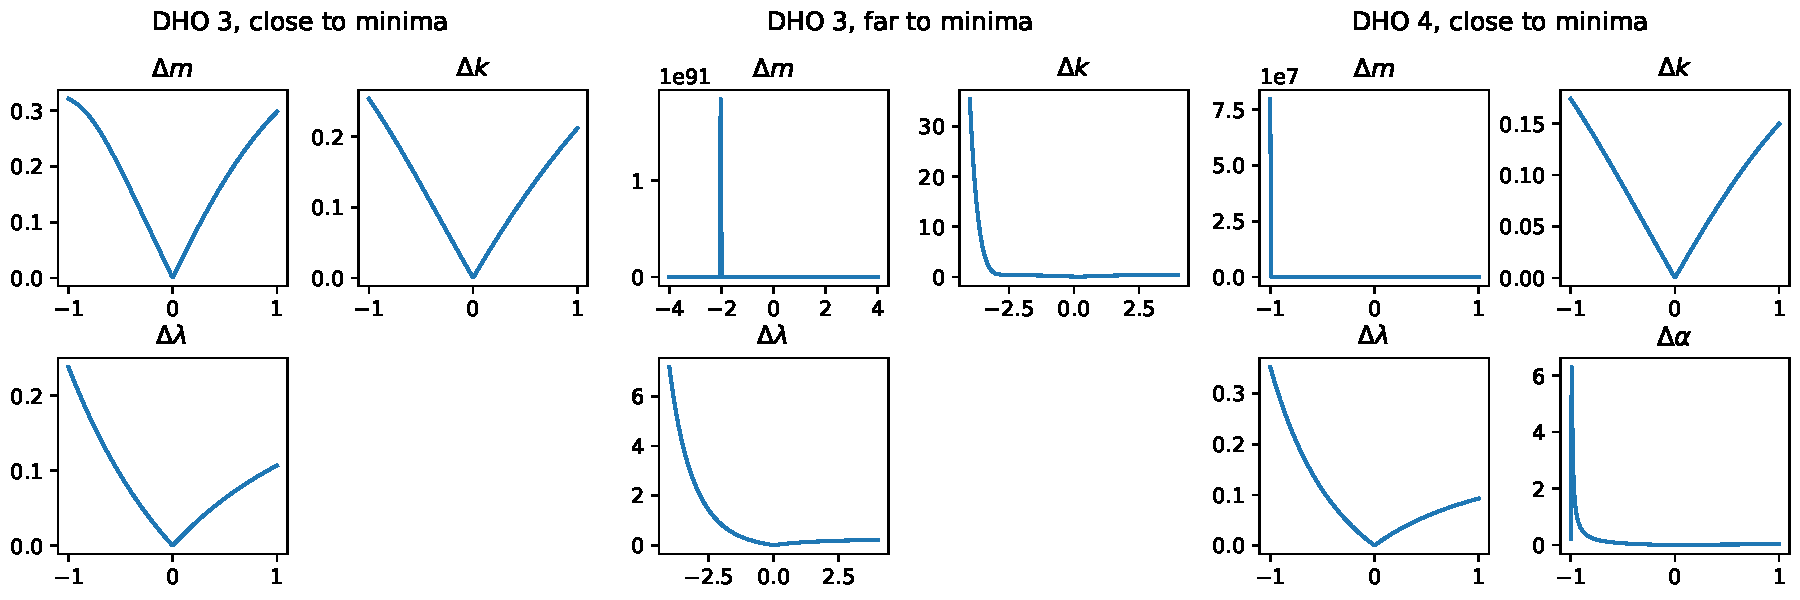
\includegraphics[width=\textwidth]{figures/loss-function-behaviour.pdf}
  \caption{The local behaviour of an equally weighted $\vbq$ and $\pi$ RMS loss function, when viewed as a function of variation in each of the embedding variables independently, with others kept fixed. We observe roughly correct behaviour in all variables bar mass $m$ and subsequently $\alpha$ for the DHO 4 embedding where $\alpha$ acts as a pre-factor for the whole non-conservative Lagrangian $\Lambda$. This behaviour is to be expected as system without mass is non-physical and explodes to infinity.}
  \label{fig:loss-function-behaviour}
\end{figure*}

\begin{table}
\label{table:loss-fns}
\centering
\caption{A list of loss functions. Key: RMS = Root Mean Squared, a standard loss function in machine learning.%; inv-exp t.w. = inverse exponential time weighting.
}
\begin{tabular}{c|p{0.5\linewidth}}
  Name & Description \\
  \hline
  Simple RMS & Sum of RMS for $\vbq$ and $\pi$ in equal weighting. \\
  RMS-$(a, b)$ & Sum of $a$ times the RMS for $\vbq$ and $b$ times the RMS for $\pi$. \\
%  RMS inv-exp t.w. & Weighting the contribution from each time-step by $e^{-t}$  \\
\end{tabular}
\end{table}

\begin{table}
\label{table:optimisation-results}
\centering
\caption{Results of optimising the chosen loss function from \tref{table:loss-fns} for $200$ initially random embeddings (distributed uniformly in $[0, 10]^n$) in the input space of the chosen embedding function, where convergence is defined as being within $\epsilon = 0.05$ of the true embedding at the end of a maximum of $250$ iterations of the optimiser. Note that for DHO 4 an additional normalisation step of dividing by $\alpha$ was applied to remove the redundancy introduced by the pre-factor in when determining if convergence had been achieved. The true embedding that was optimised towards, in DHO 3 form, was $(m = 2, k = 3, \lambda = 1)$ and systems were compared with $\Niter = 50, r = 2, \Delta t = 0.1, q_0 = 0, \pi_0 = 1$.}
\begin{tabular}{l|l|c}
  Loss function & Embedding & Convergence $\%$ \\
  \hline
  Simple RMS & DHO 3 & $33.5\%$ \\
  Simple RMS & DHO 4 & $97.5\%$ \\
  RMS-$(2, 1)$ & DHO 4 & $98\%$ \\
  RMS-$(0, 1)$ & DHO 4 & $0\%$ \\
%  RMS inv-exp t.w. & DHO 3 &
\end{tabular}
\end{table}


\subsection{PINNs and Approximating Damped Harmonic Oscillators}

Finally, we applied these techniques to a PINN. For our initial explorations in this space, we focused on fitting to systems of damped harmonic oscillators as has been the through line of the work thus far. We chose the 3-parameter DHO embedding over the 4-parameter embedding with a pre-factor as while DHO 4 was more effective when subject to direct gradient descent, we were concerned that the additional redundant embedding parameter would make learning the systems more complex and error-prone.

The dataset used in training ($N \approx 5 \times 10^5$) was a mixed selection. Primarily it was comprised of uniformly distributed embeddings within the subset of the physical region of the embedding space (positive embedding values). In addition a fraction, approximately $5 \%$ for both, of the spring and damping constants were set to zero to ensure that the model was exposed to non-damped simple harmonic motion and kinetic energy only systems.

For PINN training, accounting for the increased complexity of the optimisation problem now being with respect to the parameters of the model, we made two alterations to our loss functions. First, we added a strong weight against non-physical negative embedding values in our loss function, taking the form of,

\begin{equation}
  f(e_i) = \begin{cases}
  	0 & e_i \ge \delta \\
  	\exp{-\gamma e_i} & e_i < \delta 
  \end{cases}
\end{equation}

where $\delta = −0.1$ is a tolerance to allow for zero to be a non-penalised output and $\gamma \approx 10$ is the strength of the penalisation. This was done as the non-physical behaviour of negative embedding values is less visible when considering the larger whole model optimisation problem.
In addition, we also experimented with capping the values of the loss at large values to mitigate overflows when dealing with particularly bad fits, such as the initially random initialised weights before any training had commenced. Both of these alterations notably improved training stability and decreased the probability of floating-point related errors.

Model training was done in batches and was prone to explosion possibly due to the non-convexity in some regions as discussed in \sref{sec:res-lf}. Overall it was found that training could be made more stable by increasing batch sizes to $512$ from $32$, and manually tweaking learning rates and loss weightings (for example between the $\vb q$ and $\pi$ RMS terms where more progress was made with weighting towards $\vbq$ error to counteract observed larger tendency for error in this term) as training progressed.

Other loss functions, such as RMS in $\pi$ only (RMS-(0, 1) in \tref{table:optimisation-results}), were once again investigated. This initially looked promising, producing good losses on the order of $10^{-4}$, however on further inspection it was found that these resulted from a finding a false minima of $m \approx k \approx \lambda$, highlighting the complexity of the embedding space in representing physical systems. This also underlined the utility of the previous direct embedding space optimisation done prior in informing us about the behaviour of the loss function itself.

By the training's conclusion we obtained an absolute RMS error of $\pm 5 \times 10^{-2}$ in $\vbq$ and $\pm 1 \times 10 ^{-1}$ in $\pi$. This model was able to predict systems with some accuracy, clearly able to fit to certain features as shown in \fref{fig:model-prediction}.

\begin{figure}[t]
  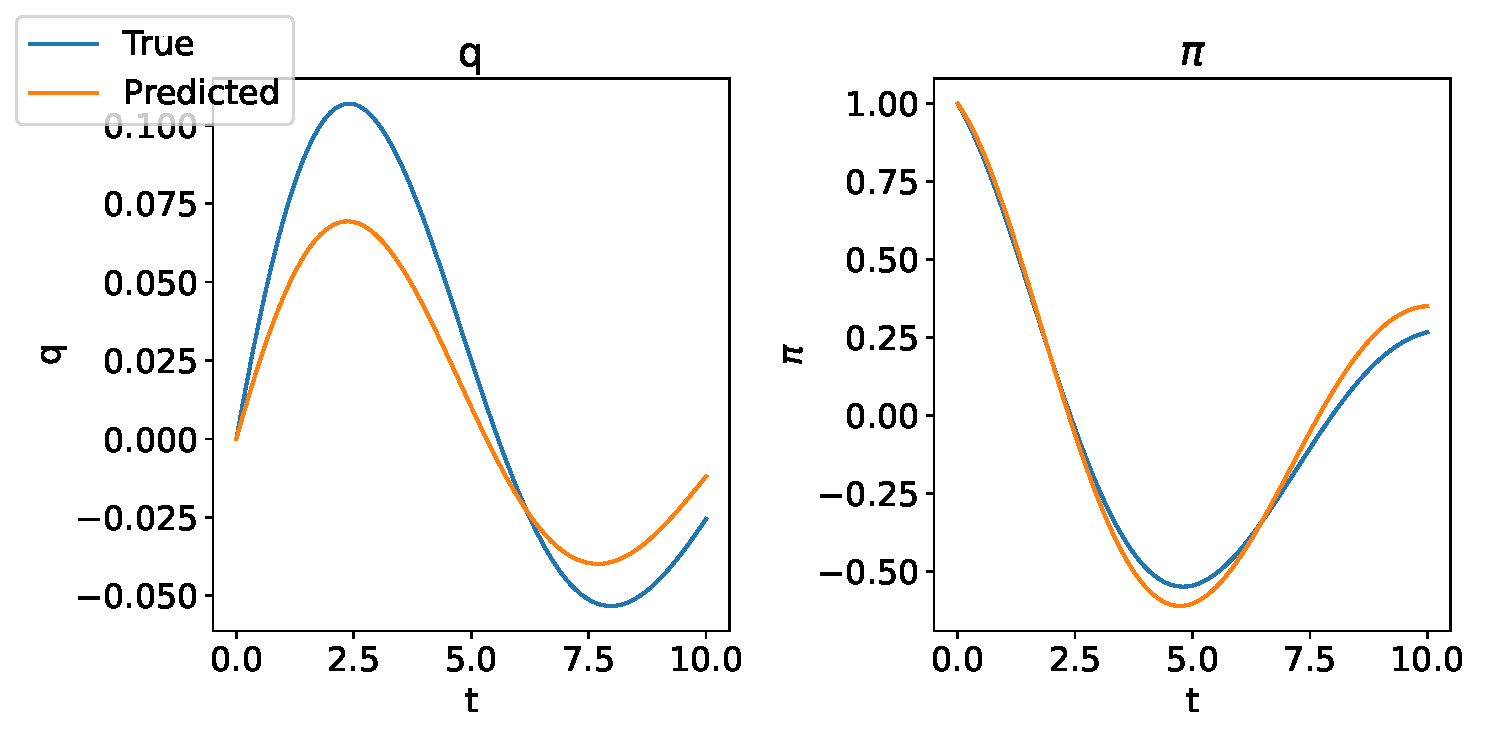
\includegraphics[width=\columnwidth]{figures/model-predictions.pdf}
  \caption{A comparison of the behaviour of a Lagrangian embedding predicted by a PINN. True embedding, $(m = 6, k = 2, \lambda = 3)$, predicted embedding, $(m = 9.401553,  k = 3.3729377, \lambda = 3.9162085)$.}
  \label{fig:model-prediction}
\end{figure}



\section{Discussion}

\subsection{\SI{}}

We have presented a number of results on the performance characteristics of the \updimpl{} of the \SI{} method when applied to physical problems which warrant additional discussion to place them in context.

Starting with the effect of changing the method order $r$, as presented in \fref{fig:dho-r-runtime}, the roughly constant behaviour observed and expected to continue for higher values of $r$ as this reflects very little change in the size of the underlying work (due to data-size and calculation cost) involved in the integration process. This coupled with the ability to split long integration runs (high $\Niter$ values) into multiple successive runs means that with careful management of errors, we should be able to the degradation to linear performance observed in \fref{fig:dho-n-runtime} for $\Niter > 10^7$ where currently internal arrays become greater than 1Gb in size possibly hitting JAX de-optimisation.

It is important to note however that in the high order domain $r \gtrsim 40$ the computation of the derivative matrix, given in Equation \eqref{eq:dij}, begins to fail as we encounter issues with the \texttt{float64} floating point precision used in JAX calculations. Unfortunately, this is unavoidable as it is the maximum precision offered by JAX. Nonetheless, this limitation can be mitigated, whilst retaining the desired error characteristics, by employing alternative strategies, such as reducing the time step or using a higher-order method with a lower value.

Overall however this approach is made more fruitful by noting that we can avoid the fixed cost entirely if we reuse the same of form non-conservative Lagrangian. This allows us to vary not only initial conditions, for example exploring the same system in different circumstances or restarting after multiple runs, but also sample across a range of physical parameters (such as those parameterising the DHO 3 embedding as defined in Equation \eqref{eq:dho-sys-embedding}). In particular this scaling without fixed costs applies effectively to systems composed of many repeated sub-systems such as field theory or molecular dynamics simulations \cite{tuckermanUnderstandingModernMolecular2000b}.

Further, as shown in \fref{fig:dho-n-runtime}, we observe a transient increase in runtime over the range $r \in [7, 9]$. This phenomenon is repeatable and its origin is uncertain. However, informed by the size of the quadrature array being $r + 2$, we suspect that this behaviour is due to optimisation cliffs in the JAX internal code as we transition between two internal implementations optimised for small vs large array sizes. Finally, it is important to consider that for less trivial systems, where evaluating the Lagrangian may have its own performance impacts, may require further analysis and optimisation. This class of complexity management however is a well studied and understood trade off.

Looking forwards, we noted that the use of fixed time steps in the method limits our ability to maintain energy and momentum fractional error bounds. Moving to an adaptive time step approach would be a promising avenue for improvement in future work.

\subsection{PINN, Current and Future}

The trained neural network represents a promising first step in predicting non-conservative Lagrangians from observational data successfully capturing the general characteristics of the data.
During our experiments, we frequently observed predicted embeddings with values of roughly correct proportion, but off by a constant factor. This suggests that the 4 parameter embedding or other normalisation method may have been useful as the system was unable to move past this local minima in phase space, representing a sufficiently similar physical system.
This poses questions on the handling of degeneracy in our Lagrangian space where multiple Lagrangians can result in the same physical system, especially within the image of any chosen embedding function, as this degeneracy will present issues when optimising within the space.

Furthermore, we noted that the model was substantially more accurate with comparatively high masses. We theorise that this may be due to difficulties in fitting larger values of $\vbq$, possibly indicating the need for a larger and more varied dataset. It is important to acknowledge that this was a simplified test network, and we anticipate that future work will achieve improvements by utilising a larger parameter count and datasets.

To enhance the model's performance, incorporating physically known a priori information into the loss function may be beneficial. For example, a stricter restriction on non-negativity for the DHO 3 parameters could be implemented by first taking the absolute value of the outputs as inputs to the Slimpletic Integrator. However, this approach presents a trade-off, as we specialise towards particular physical systems where we have more physical knowledge, but create models that are less widely applicable. Identifying physical laws that can be enforced in the Lagrangian would be a fruitful avenue for future research.

In the same vein, a suitably trained neural network could be constructed using this method to identify symmetries in observational data or recognise patterns it has previously been exposed to in new observational data. This suggests potential applications in domains such as astrophysics, where there is a large availability of data to train a model, but also difficulties in obtaining a complete dataset for any one experiment.

\section{Conclusion}

In this paper we have put forward a more optimal implementation of the Slimpletic Integrator, which is capable of scaling to large scale physical simulations while preserving bounded fractional error in the energy. We have shown this implementation has applications in the construction of a loss function for physics informed neural networks, and presented a simple model which shows that this approach has promise for identifying non-conservative Lagrangians from observational data. More work is required to explore better encodings of physical invariants in the loss function and model structure.
